\chapter{Valg av prosess}
Dette kapittelet skal beskrive og begrunne utviklingsmetodikken som ble valgt for utviklingen av masteroppgaven. Flere kjente utviklingsmetodikker ble undersøkt og vurdert mot hverandre for å finne det som egnet seg best til dette prosjektet.

% \section{Forskningsmetode}
% Kunnskap om utfordringene og problemstillingene med å manuelt gjennomføre oppsynsturer for sau på utmarkbeite i dag ble presentert for utviklerne av professor Hvasshovd. Han har opparbeidet seg erfaring ved utføre oppsynsturer i Trøndelag over mange år. Denne kompetansen stilte professor Hvasshovd til rådighet for utviklerne ved å ha ukentlige møter der han utdypet dagens prosess for oppsynsturer samtidig som han ha veiledning for selve utformingen av applikasjonen og rapporten. Hvasshovds innsikt og informasjon ble brukt som utgangspunkt for videre litteratursøk via Internett for å kunne utarbeide nok kunnskap for å utarbeide problemstillingen og bakgrunnen for prosjektet beskrevet i kapt. \ref{bakgrunn}. 

\section{Utviklingsmetodikk}
Innenfor utvikling av programvaresystemer vil utviklingsmetodikk referere til prosessen med å planlegge, utvikle, teste og distribuere et prosjekt \cite{rachieleSoftwareDevelopmentMethodologies2018} der målet er å lage programvare. Med andre ord betyr det en bestemt metodikk for å strukturere prosessen og arbeidet for å effektivisere utviklingsprosessen samt implementere et produkt av høyere kvalitet. Hvilken metodikk som har vært fremtredende innen programvareutvikling har endret seg over tid og med utviklingen av nye programmeringspråk, rammeverk, verktøy og omfanget av programvaresystemene. I dag finnes det mange ulike utviklingsmetodikker som har sine styrker og svakheter ut i fra prosjektets mål og omfang. Videre skal to kjente utviklingsmetodikker, Vannfallsmodellen og agil utvikling, beskrives og vurderes som metodikker for prosjektet.   
\newline 
\newline 
Lenge var den linære Vannfallsmodellen den mest populære metodikken, og brukes fortsatt i dag selv om andre utviklingsmetodikker har blitt mer dominerende de siste årene \cite{WaterfallModelWhat2016}. Lignende metodikk ble først beskrevet på 1950-tallet, men Vannfallmodellen slik den er kjent i dag ble opprinnelig introdusert av Wintson Royce i 1970 \cite[~s.329]{royceManagingDevelopmentLarge1970}. I Vannfallsmodellen deles prosessen opp i sekvensielle faser som følger etter hverandre (se figur \ref{fig:waterfall-model} under), der én fase må fullføres før man kan starte på neste fase \cite{WaterfallModelSoftware}. Disse fasene og rekkefølgen på dem er \cite{royceManagingDevelopmentLarge1970}: 
\begin{enumerate}
    \item Programvarekrav - Kravene for applikasjonen analyseres og skrives ned som utgangspunkt for fremtidig utvikling \cite{WaterfallModelWhat2016}.
    \item Analyse - Systemet analyseres for å kunne lage modeller og forretningslogikken som skal brukes i applikasjonen \cite{WaterfallModelWhat2016}.
    \item Programdesign - Dekker de tekniske designkravene som programmeringsspråk, datalag, tjenester osv. \cite{WaterfallModelWhat2016}.
    \item Koding - Faktisk kildekode blir skrevet og alle modellene som ble utformet i tidligere faser implementeres \cite{WaterfallModelWhat2016}.
    \item Testing - Testere går systematisk gjennom applikasjonen og rapporterer om feil som må løses \cite{WaterfallModelWhat2016}.
    \item Operasjoner - Applikasjonen blir distribuert. Denne fasen inneholder også nødvendig vedlikehold for å holde applikasjonen funksjonell \cite{WaterfallModelWhat2016}. 
\end{enumerate}
Fordelen med Vannfallsmodellen er at den er svært enkel å forstå, både for utviklere og kunder av applikasjonen. De rigide og klart definerte fasene gjør at det er lett å lage tidslinje for leveranse og milepæler, samt at prosessen og resultatene er veldokumenterte \cite{SDLCWaterfallModel}. Vannfallsmodellen passer derfor best for mindre prosjekt der kravene er veldokumenterte, klare og fikserte fra starten av og produktdefinisjonen er stabil gjennom hele prosjektet \cite{SDLCWaterfallModel}. Ulempen med Vannfallsmodellen er at de aller fleste systemer som utvikles i dag er store, komplekse og endres stadig, noe som gjør det vanskelig å definere alle krav før utviklingen begynner \cite{SDLCWaterfallModel}. Dette har ført til at tradisjonelle og linære utviklingsmetodikker innen programvareutvikling slik som Vannfallsmodellen har i senere tid blitt erstattet av agile, iterative metodikker \cite{livermoreFactorsThatImpact2007}. 
\newline
\newline
Agil metodikk er en betegnelse for mange ulike iterative og inkrementelle utviklingsmetodikker som følger en agil filosofi, praksis og prinsipp \cite[~s.20]{rannikkoUserCenteredDesignAgile2011}. Selv om agil metodikk og lignende lettvektsprinsipper har vært i bruk siden sent 1950-tallet \cite[~s.80]{larmanAgileIterativeDevelopment2004}, var det først på 1990-tallet at agil metodikk begynte å bli utbredt \cite[~s.87]{larmanAgileIterativeDevelopment2004}. I 2001 gikk flere anerkjente personer innen utviklingsmetodikk sammen og utga dokumentet \enquote{Agile Manifesto} \cite{beckManifestoAgileSoftware2001} som en reaksjon mot tradisjonelle linære metodikker som Vannfallsmetoden og deres rigide krav om dokumentasjon \cite{livermoreFactorsThatImpact2007}. Med deres erfaring i programvarebransjen beskriver de 4 grunnleggende prinsipper for agil programvareutvikling \cite{beckManifestoAgileSoftware2001}: 
\begin{itemize}
    \item Individer og interaksjoner over prosesser og verktøy.
    \item Fungerende programvare over omfattende dokumentasjon.
    \item Kundesamarbeid over kontraktsforhandlinger.
    \item Svare på endringer over å følge en plan. 
\end{itemize}
Den høyste prioriteten er å gjøre kunden fornøyd, og med iterativ, agil utvikling kan kunden få leveranser i form av fungerende programvare kontinuerlig gjennom hele utviklingsprosessen \cite{beckPrinciplesAgileManifesto2001}.  Endringer i kravene ønskes velkommen, selv sent i utviklingstadiet \cite{beckPrinciplesAgileManifesto2001}. Den mest effektive metoden for å formidle informasjon innen utviklingteamet er via direkte kommunikasjon ansikt til ansikt, ofte daglig \cite{beckPrinciplesAgileManifesto2001}. Akkurat hvordan disse prinsippene blir fulgt i en utviklingsprosess, vil variere ut i fra hvilken agil utviklingsmetodikk som blir valgt.

\begin{figure}[H]
  \centering
  \begin{minipage}[b]{0.45\textwidth}
    \centering
    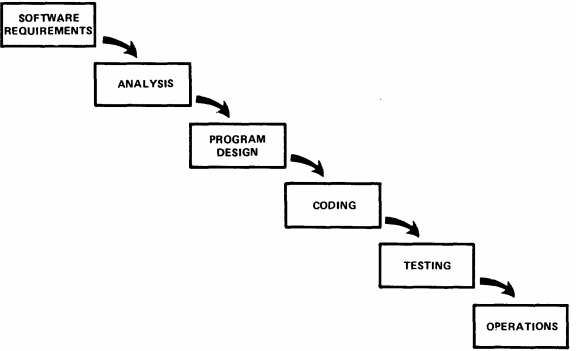
\includegraphics[scale=0.4]{Figurer/diagram/waterfall-model.png}
    \caption{Vannfallsmodellen beskrevet av Winston Royce}
    \source{\cite{royceManagingDevelopmentLarge1970}}
    \label{fig:waterfall-model}
  \end{minipage}
  \hfill
  \begin{minipage}[b]{0.45\textwidth}
    \centering
    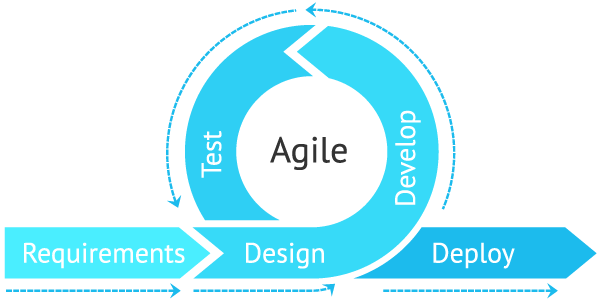
\includegraphics[scale=0.3]{Figurer/diagram/agile-dev.png}
    \caption{Modell over agil utvikling}
    \source{\cite{WhyAgileImportant2020}}
    \label{fig:agile-dev}
  \end{minipage}
\end{figure}
\noindent
Det ble bestemt i starten av utviklingsprosessen å gå for en agil utviklingsmetodikk framfor den mer tradisjonelle Vannfallsmetoden. Selv om utviklingsteamet bare består av to personer og applikasjonen har et nokså snevert og spesifisert omfang, var ikke kravspesifikasjonen fastsatt fra starten av. Mange av funksjonene og valg av teknologi ble tatt underveis i prosjektets løp ved å ha ukentlige møter sammen med professor Hvasshovd. Det var et behov å kunne tilpasse seg gjennom prosjektet. Ettersom utviklerne i tillegg hadde mer erfaring med agil metodikk, var slik metodikk bedre egnet for hele prosjektet, både for fordypningsprosjektet og masteroppgaven.

\subsection{Valg av agil metodikk}
Eksempler på noen av de mest kjente agile metodikkene er Scrum \cite{HomeScrumOrg}, Kanban og Extreme Programming \cite{wellsExtremeProgrammingGentle2009}. I dette prosjektet ble Scrum og Kanban vurdert. 
\newline
\newline
Scrum, som for alvor tok av etter boken \enquote{Agile software development with Scrum} \cite{schwaberAgileSoftwareDevelopment2002} i 2002, kjennetegnes ved at både kunder og utviklingsteam får roller med et bestemt ansvarsområde samt en rekke artefakter og hendelser som gjentas over prosjektets løp \cite{WhatScrum}. Prosjektet gjennomføres ved å deles inn i kortere iterasjoner kalt \textit{sprinter} \cite{WhatScrum} som er en fast leveransesyklus på 1-4 uker \cite{nesKortIntroduksjonTil2019}. Produkteierens ansvar er å lage en prioriert liste over produktets ønskede funksjonalitet, kalt \textit{backlog}, som det blir tatt utgangspunkt i når man skal lage en egen \textit{backlog} for \textit{sprinten} som skal gjennomføres \cite[~s.24]{rannikkoUserCenteredDesignAgile2011}. Utviklerteamet har ansvar for å implementere og potensielt levere et produkt eller funksjon for hver sprint og oppdatere \textit{backloggen} underveis ved hjelp av en Scrum-tavle som visualiserer oppgavene \cite[~s.24]{rannikkoUserCenteredDesignAgile2011}. Hver dag møtes utviklerne for korte \textit{standup}-møter der de forteller hva som har blitt gjort og hva som skal gjøres for dagen, slik at alle er oppdaterte \cite{WhatScrum}. Etter hver \textit{sprint} gjennomføres et refleksjonsmøte for å se hva som kan forbedres i prosessen til neste \textit{sprint} \cite{WhatScrum}. I tillegg får en av utviklerene en ekstra rolle som Scrum-master som skal sørge for at alle i teamet forstår og følger Scrum-praksis \cite[~s.24]{rannikkoUserCenteredDesignAgile2011}. 
\newline
\newline
Kanban oppstod på 1940-tallet da Toyota begynte å bruke det i deres fabrikker for å optimalisere arbeidsflyten. På 2000-tallet ble prinsippene utviklet hos Toyota overført til programvareutvikling \cite{radiganKanbanBriefIntroduction}. Det er en agil metodikk med et par likheter til Scrum. Det brukes blant annet også en tavle for å vise \textit{backlog}, pågående arbeidsoppgaver og utførte oppgaver eller andre egendefinerte lister \cite{radiganKanbanBriefIntroduction}. Kanban har et spesielt fokus på å optimalisere arbeidsflyt, maksimere effektivitet og unngå flaskehalser \cite{radiganKanbanBriefIntroduction}. Derfor benyttes det ikke tidsbestemte \textit{sprinter} slik som i Scrum, men en kontinuerlig flyt av arbeid og distribusjon \cite{radiganKanbanBriefIntroduction}. Det er heller ingen faste roller for de involverte i prosjektet. Pågående oppgaver for hver arbeidskategori blir begrenset slik at utviklerne ikke påtar seg for mange oppgaver samtidig og stagnerer fremdriften i prosjektet \cite{radiganKanbanBriefIntroduction}. Om antall pågående arbeidsoppgaver er på den fastsatte maksgrensen for påbegynte oppgaver, må en utvikler hjelpe til med de påbegynte oppgavene før en ny oppgave kan startes på \cite{radiganKanbanBriefIntroduction}. 
\newline
\newline
Selv om utviklerne hadde mest erfaring med å utvikle med Scrum både i skole- og arbeidssammenheng, ble det sett på som lite hensiktsmessig med tanke på at det bare var to utviklere i prosjektet. Det ville vært vanskelig å utfylle alle arbeidsrollene og ført til unødvendig bruk av tid med \textit{standup-} og refleksjonsmøter når utviklerne under så og si hele utviklingsprosessen var i samme rom og kunne holde hverandre oppdatert kontinuerlig. Å utvikle i \textit{sprinter} ble også valgt bort ettersom det hadde vært tidkrevende å planlegge disse sammen med produkteier professor Hvasshovd annen hver uke. Kanban ble derfor et naturlig valg for dette prosjektet med mulighet for kontinuerlig flyt, fravær av bestemte arbeidsroller og visualisering samt begrensning av arbeidsoppgaver som gjorde det enklere å få øye på flaskehalser i utviklingsprosessen. 

\subsubsection{Trello}
En essensiell del av Kanban er tavlen som visualiserer arbeidsoppgavene. Dette kan være en fysisk liste med klistrelapper eller digitale tavler. Under dette prosjektet ble samhandlingsverktøyet Trello \cite{Trello} benyttet ettersom det kunne bli brukt i sanntid av begge utviklerne og la til rette for bruk av fargekoder slik at oppgavene kunne kategoriseres både for utvikling av programkode, skriving av oppgaven og andre egendefinerte kategorier. Det faktum at tavlen kunne oppdateres i sanntid gjorde også enklere for utviklerne å være oppdatert på hva den andre personen arbeidet med i de periodene utviklerne hadde hjemmekontor hver for seg. Utviklerne valgte å sette maksgrensen for påbegynte arbeidsoppgaver til tre, som det er mulig å se i figuren under i listen WIP (Work in Progress). 
\begin{figure}[H]
\centering
\captionsetup{width=.8\linewidth}
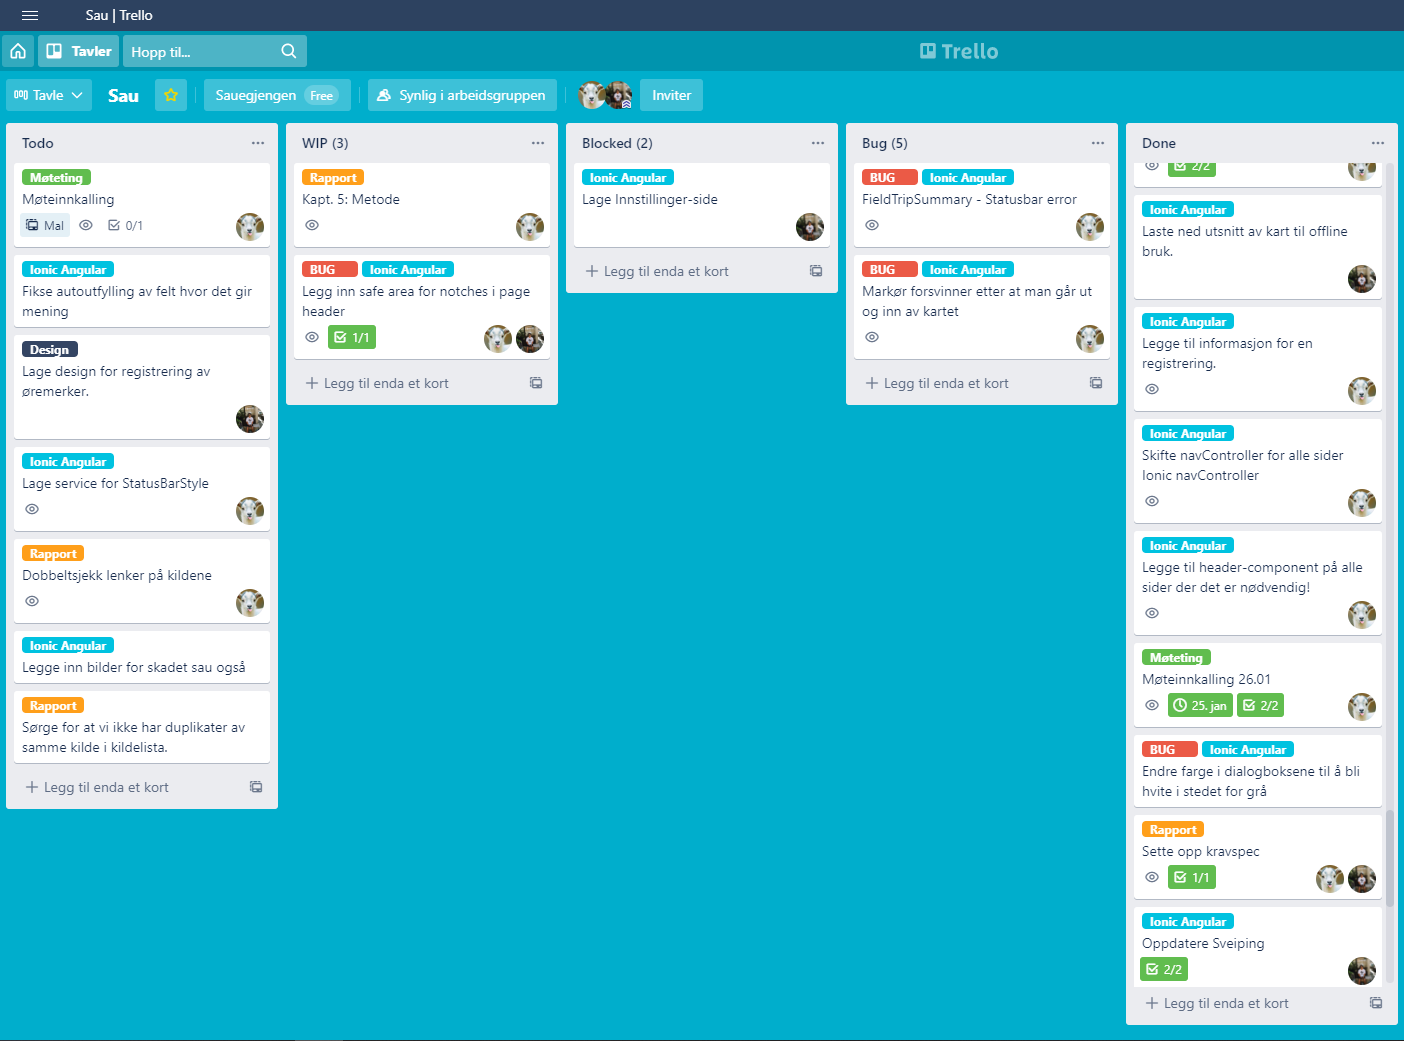
\includegraphics[scale=0.4]{Figurer/Bilder/trello.png}
\caption{Skjermbilde av Trello-tavlen under prosjektet.}
\label{fig:trello}
\end{figure}

\section{Konklusjon}
% Forskningsmetoden brukt i dette prosjektet for å innhente informasjon og kunnskap om oppsyn av sau ble gjennomført med ukentlige møter med veileder og litteratursøk på internett.
Det ble bestemt å bruke en agil utviklingsmetodikk og ikke den mer tradisjonelle Vannfallsmodellen. Dette er grunnet at kravspesifikasjonene ikke var satt før prosjektets start men utviklet underveis, og agil metodikk er svært tilpasningsdyktig i motsetning til Vannfallsmodellen som er mer rigid. Av mange ulike agile metodikker falt valget på Kanban som passet best det et lite utviklingsteam med dets kontinuerlige flyt av arbeid, fravær av bestemte roller for de involverte i prosjektet samt visualisering og begrensning av arbeidet som vises på en tavle.  Samhandlingsverktøyet Trello ble benyttet som en digital Kanban-tavle.